% Options for packages loaded elsewhere
\PassOptionsToPackage{unicode}{hyperref}
\PassOptionsToPackage{hyphens}{url}
%
\documentclass[
]{article}
\usepackage{lmodern}
\usepackage{amssymb,amsmath}
\usepackage{ifxetex,ifluatex}
\ifnum 0\ifxetex 1\fi\ifluatex 1\fi=0 % if pdftex
  \usepackage[T1]{fontenc}
  \usepackage[utf8]{inputenc}
  \usepackage{textcomp} % provide euro and other symbols
\else % if luatex or xetex
  \usepackage{unicode-math}
  \defaultfontfeatures{Scale=MatchLowercase}
  \defaultfontfeatures[\rmfamily]{Ligatures=TeX,Scale=1}
\fi
% Use upquote if available, for straight quotes in verbatim environments
\IfFileExists{upquote.sty}{\usepackage{upquote}}{}
\IfFileExists{microtype.sty}{% use microtype if available
  \usepackage[]{microtype}
  \UseMicrotypeSet[protrusion]{basicmath} % disable protrusion for tt fonts
}{}
\makeatletter
\@ifundefined{KOMAClassName}{% if non-KOMA class
  \IfFileExists{parskip.sty}{%
    \usepackage{parskip}
  }{% else
    \setlength{\parindent}{0pt}
    \setlength{\parskip}{6pt plus 2pt minus 1pt}}
}{% if KOMA class
  \KOMAoptions{parskip=half}}
\makeatother
\usepackage{xcolor}
\IfFileExists{xurl.sty}{\usepackage{xurl}}{} % add URL line breaks if available
\IfFileExists{bookmark.sty}{\usepackage{bookmark}}{\usepackage{hyperref}}
\hypersetup{
  pdftitle={A Mosquito Problem},
  pdfauthor={Chris Berg},
  hidelinks,
  pdfcreator={LaTeX via pandoc}}
\urlstyle{same} % disable monospaced font for URLs
\usepackage[margin=1in]{geometry}
\usepackage{graphicx,grffile}
\makeatletter
\def\maxwidth{\ifdim\Gin@nat@width>\linewidth\linewidth\else\Gin@nat@width\fi}
\def\maxheight{\ifdim\Gin@nat@height>\textheight\textheight\else\Gin@nat@height\fi}
\makeatother
% Scale images if necessary, so that they will not overflow the page
% margins by default, and it is still possible to overwrite the defaults
% using explicit options in \includegraphics[width, height, ...]{}
\setkeys{Gin}{width=\maxwidth,height=\maxheight,keepaspectratio}
% Set default figure placement to htbp
\makeatletter
\def\fps@figure{htbp}
\makeatother
\setlength{\emergencystretch}{3em} % prevent overfull lines
\providecommand{\tightlist}{%
  \setlength{\itemsep}{0pt}\setlength{\parskip}{0pt}}
\setcounter{secnumdepth}{-\maxdimen} % remove section numbering

\title{A Mosquito Problem}
\author{Chris Berg}
\date{}

\begin{document}
\maketitle

\emph{This problem was written by George Evans and comes from the
University of Oregon core macroeconomics exam, in July of 2013.}

\hypertarget{setup}{%
\subsection{Setup}\label{setup}}

Imagine that at time \(t\) there are \(M_t > 0\) mosquitos carrying a
deadly novel influenza virus around an economy with labor force
\(L_t > 0\). We are given the following equations of reproduction for
the labor force, and the mosquito population:

\begin{align}

\dot{M} &= (\phi - \sigma)M_t - Z_t \\
\dot{L} &= nL_t - \phi M_t

\end{align}

Here, \(\phi > 0\) is the growth rate of the virulent mosquito
population and \(\sigma > 0\) is the mortality rate of the mosquitos (at
least, the ones with the virus). The labor force grows at rate
\(n > 0\). \(Z_t > 0\) can be thought of, in general, as a good which
abates the mosquitos who have the virus (i.e.~mosquito repellant, or
even as general as the disposal of food which the mosquitos feast upon).
The abatement good and the consumption good \(C_t > 0\) can each be
produced using a production technology with unit labor requirements
\(a,b > 0\) \footnote{The careful observer will notice this equation is
  actually the production possibilities frontier for a given labor
  force.}:

\begin{align}

aZ_t + bC_t = L_t

\end{align}

We can take initial values \(M(0) , L(0)\) as given.

\hypertarget{task-a}{%
\subsection{Task A}\label{task-a}}

\begin{enumerate}
\def\labelenumi{\arabic{enumi}.}
\tightlist
\item
  \emph{Show, for a suitable constant \(k\) depending on the parameters,
  that if \(x = \frac{L}{M}\) and \(z = \frac{Z}{M}\)\ldots{}}
\end{enumerate}

\[ \dot{x} = (z-k)x - \phi \]

\textbf{Answer:}

Start off by noticing that given the definition of \(x\), we can write
\[\dot{x} \equiv \frac{dx}{dt} =  \frac{dLM^{-1}}{dt} = \frac{\dot{L}M - L\dot{M}}{M^2} \]

Breaking the difference apart and substituting yields \begin{align} 

\dot{x} &= \frac{nL - \phi M}{M} - \frac{L}{M}((\phi - \sigma) - z) \\
        &= nx - (\phi - \sigma)x + zx - \phi \\
        &= (z - ((\phi - \sigma )- n) )x - \phi \\
\end{align}

Therefore \(\dot{x} = (z-k)x - \phi\) for \(k = (\phi - \sigma) - n\) as
the problem asks for.

\begin{enumerate}
\def\labelenumi{\arabic{enumi}.}
\setcounter{enumi}{1}
\tightlist
\item
  \emph{Suppose policy aims to set \(z = \bar{z} > 0\) constant over
  time. What would happen to \(x\) over time if \(k>0\) and
  \(0<k<\bar{z}\)?}
\end{enumerate}

It's easy to see that for \(\dot{x} = (z-k)x - \phi\) and \((z-k)<0\) by
assumption, then given our other assumption that \(x,\phi > 0\) it must
be that \(\dot{x} < 0 \ \forall \ t\). Thus the ratio of the human labor
force (or human population as it were) to virulent mosquitos goes down
forever, as the mosquitos/virus overtakes the human labor force.

\hypertarget{task-b}{%
\subsection{Task B}\label{task-b}}

Disclaimer: The answer for several parts of this task admittedly go
\emph{much further} than requested in the question, in order to
drill-down into what all is happening behind the scenes with this
problem.

Now we are given \(c_t = \frac{C_t}{L_t}\) and told to imagine a planner
who wishes to maximize

\[U = \int^{\infty}_{0} e^{-\rho t} u(c_t) dt\]

subject to the familiar state constraint

\[ \dot{x} = (z-k)x - \phi\]

\begin{enumerate}
\def\labelenumi{\arabic{enumi}.}
\tightlist
\item
  \emph{Using \(c = 1/b - \frac{az}{bx}\) and treating \(x\) as the
  state variable and \(z\) as the control, write down the Hamiltonian
  and the first-order conditions for an optimum.}
\end{enumerate}

\textbf{Answer:}

We are given the state to be \(z\) so the first order of business is to
substitute the given formula for \(c\) (which can even be derived from
the production possibilities frontier equation for given \(L\)) into the
utility function when we are forming the Hamiltonian:

\[ \mathcal{H_t} = u\left(\frac{1}{b} - \frac{a}{bx_t}z_t \right) + \lambda_t((z_t-k)x_t - \phi)\]

The first-order conditions for an optimum in this problem\footnote{Ignoring
  the second-derivative issue by assuming concavity of \(u(\cdot)\)} are
given by the following system of equations

\begin{align}

\frac{\partial u}{\partial c_t}\frac{d c_t}{d z_t} + \lambda_t x_t &= 0 \\

\dot{\lambda} = \rho \lambda_t - \frac{\partial \mathcal{H_t}}{\partial x_t} &= \rho \lambda_t - \left[\frac{\partial u}{\partial c_t}\frac{d c_t}{d x_t} + \lambda_t (z_t - k) \right] \\

\lim_{t \to \infty} e^{-\rho t}\lambda_t x_t &= 0 

\end{align}

One thing we'll need is \(d c_t/d z_t\) and \(d c_t/d x_t\) to solve
this. Let's also just call \(u' \equiv \frac{\partial u}{\partial c_t}\)

\begin{align}

\frac{d c_t}{d z_t} &= -\frac{a}{bx_t} \\
\frac{d c_t}{d x_t} &= (-1)\left(-\frac{az_t}{bx_t^2}\right)  \\
&= \frac{d c_t}{d z_t}\left(-\frac{z_t}{x_t}\right)

\end{align}

With these, let's substitute and re-write the first-order conditions:

\begin{align}
\left( -\frac{a}{bx_t}\right)u' + \lambda_tx_t &= 0 \\
\Rightarrow \lambda_t = \frac{a}{bx_t^2}u' &= \frac{d c_t}{d x_t}\frac{u'}{z_t} \\
\dot{\lambda} = \rho \lambda_t - \left[ (\lambda_t z_t) + \lambda_t z_t - \lambda_t k \right] &= (\rho - 2z_t + k)\lambda_t \\
\Rightarrow \frac{\dot{\lambda}}{\lambda_t} &= \rho - 2z_t + k

\end{align}

Notice the substitution made for \(u'\frac{d c_t}{d x_t}\) on the third
line. To finish out the model solution, all we need is a closed-form
expression for \(\dot{\lambda} \equiv \frac{d\lambda}{dt}\). For this
particular model where \(z_t\) is the control, this is about as painless
as pulling your own tooth, and so George doesn't ask for this on the
actual exam. We shall not be deterred so easily however. I'll mostly
drop time subscripts from here on out.

\begin{align}

\lambda_t = \frac{a}{b}\frac{u'(z_t , x_t)}{x_t^2} \Rightarrow \frac{d\lambda}{dt} &= \frac{a}{b}\left[\frac{(d/dt \ u')x_t^2 - (d/dt \ x_t^2)u'}{x_t^4}\right] \\
&= \frac{a}{b}\left[\frac{u''\cdot(\frac{d c}{d z}\dot{z} + \frac{d c}{d x}\dot{x})x_t^2 - 2u'x_t\dot{x}}{x_t^4} \right] \\ 
&= \frac{a}{bx_t^2}\left[\frac{u''\frac{d c}{d z}(\dot{z} - \frac{z}{x}\dot{x})x_t^2 - 2u'x_t\dot{x}}{x_t^2} \right] \\
\Rightarrow \frac{\dot{\lambda}}{\lambda} = \frac{\frac{a}{bx^2}(u''\frac{d c}{d z}(\dot{z} - \frac{z}{x}\dot{x})x_t^2 - 2x_tu'\dot{x})/x_t^2}{\frac{a}{bx^2}u'} &= \frac{d c}{d z}\frac{u''}{u'}(\dot{z} - \frac{z}{x}\dot{x}) - 2\frac{\dot{x}}{x}

\end{align}

And we have it-- an expression for \(\frac{\dot{\lambda}}{\lambda}\)
that we can substitute into the first-order condition:
\[ \frac{\dot{\lambda}}{\lambda} = \frac{a}{bx}\frac{u''}{u'}\left(z\frac{\dot{x}}{x} - \dot{z}\right) - 2\frac{\dot{x}}{x} \]

As we substitute this into the left-hand side of the first-order
condition derived earlier, we'll divide both sides of the FOC by \(z\).

\[\frac{a}{bx}\frac{u''}{u'}\left(\frac{\dot{x}}{x} - \frac{\dot{z}}{z}\right) - \frac{2}{z}\frac{\dot{x}}{x} = \frac{\rho + k}{z} - 2\]

It will be helpful here to substitute \(\dot{x} = (z-k)x - \phi\) at
this point.

\begin{align}

\frac{a}{bx}\frac{u''}{u'}\left[z - k - \frac{\phi}{x} - \frac{\dot{z}}{z}\right] - \frac{2}{z}\left[(z-k) - \frac{\phi}{x}\right] &= \frac{\rho}{z} + \frac{k}{z} - 2 \\
\Rightarrow \frac{a}{bx}\frac{u''}{u'}\left[ z - k - \left( \frac{\dot{z}}{z} + \frac{\phi}{x}\right) \right] + \frac{2 \phi}{zx} &= \frac{(\rho - k)}{z} \\
\Rightarrow \frac{a}{bx}\frac{u''}{u'}\left[ z - k - \frac{\dot{z}}{z} - \frac{\phi}{x} \right] &= \frac{(\rho - k) - 2\phi/x}{z} \\
\Rightarrow \frac{u''}{u'}\left[ z - k - \frac{\dot{z}}{z} - \frac{\phi}{x} \right] &= \frac{b}{a}\left[\frac{(\rho - k)x - 2\phi}{z}\right] \\
\Rightarrow z - k - \frac{\dot{z}}{z} - \frac{\phi}{x} &= \frac{b[(\rho - k ) - 2\phi]}{az\frac{u''}{u'}} \\
\Rightarrow \frac{\dot{z}}{z} &= z - \frac{\phi}{x} - k - \frac{b(\rho - k)}{a\frac{zu''}{xu'}} - \frac{2b\phi}{az\frac{u''}{u'}} \\
\Rightarrow \frac{\dot{z}}{z} &= z - \left( \frac{\phi}{x} + \frac{\phi}{x}2b\frac{xu'}{azu''} \right)- b(\rho - k)\frac{xu'}{azu''} - k

\end{align}

Now that we've set-up and even solved the Hamiltonian, let's turn to the
second part of this questuon before we totally close this part of the
model off.

\begin{enumerate}
\def\labelenumi{\arabic{enumi}.}
\setcounter{enumi}{1}
\tightlist
\item
  \emph{For suitable U it can be shown that the first order conditions
  imply} \[\frac{\dot{z}}{z} = z - (1+\xi)\phi x^{-1} - A\] \emph{for
  constants A and \(\xi>0\). (You are not asked to show this). Compute
  the slopes dz/dx for the two curves \(\dot{x} = 0\) and
  \(\dot{z} = 0\).}
\end{enumerate}

George ultimately gave us the biggest hint here; ``For suitable
U\ldots{}'' We very often see utility functions for which
\[\frac{cu''(c)}{u'(c)} = \frac{1}{s'}\] for a constant
\(s'\).\footnote{These are called ``constant relative risk aversion''
  utility functions.} This function will need to be similar, with slight
differences though. Given our equation derived from the production
possibilities frontier, \(\frac{az}{x} = (1-bc)\), we could posit that

\[ \frac{azu''}{xu'} = \frac{1}{s} = \text{constant}\]

This would be fulfilled, for instance, if \(u = c - \gamma c^2\) and
\(b = 2\gamma\). Regardless, if we take this to be fulfilled in a manner
similar to the hint in the question, then for \(\xi = 2bs\) and
\(A=b(\rho - k)s + k\) then sure enough,

\[\frac{\dot{z}}{z} = z - (1+\xi)\frac{\phi}{x} - A\]

Adopting this notation going forward, we can see from setting
\(\dot{x} = 0 = (z - k)x - \phi\) we'll have
\(\tilde{z}= \frac{\phi}{\tilde{x}} + k\) and then

\[ \left. \frac{dz}{dx} \right\rvert_{\dot{x} = 0} = -\frac{\phi}{x^2}\]

Likewise if we set \(\dot{z} = 0 = z(z - (1+\xi)\frac{\phi}{x} - A)\)
then we get \(\hat{z}= (1+\xi)\frac{\phi}{\hat{x}} + A\) and in that
case,

\[ \left. \frac{dz}{dx} \right\rvert_{\dot{z} = 0} = -(1+\xi)\frac{\phi}{x^2}\]
3.\emph{Assuing a unique positive steady-state(\bar\{x\},\bar\{z\}),
shetch the phase diagram is (x,z) space. Indicate the optimal path from
initial \(x(0)\) to the steady state.}

I can't over-emphasize the importance of being able to quickly assess
phase diagrams. Many an exam score has been harmed by confusion over
drawing them! I've provided a fleshed-out phase diagram of this problem
below, called a ``stream plot,'' which is similar to a vector plot of a
phase diagram except for instead of point vectors, there are many
different diverging paths drawn starting at various points. You'll need
to fill-in the saddle path on your own, but the figure below should
offer intuition for how this model's phase diagram works.

\begin{center}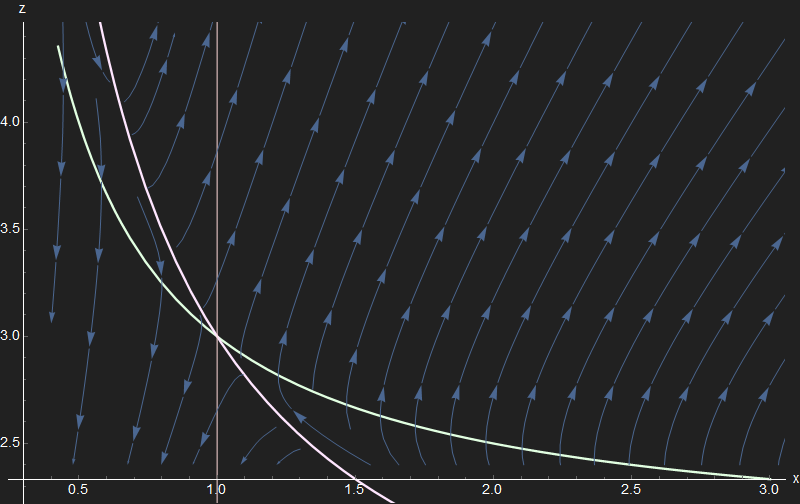
\includegraphics[width=0.8\linewidth,height=0.8\textheight]{phaseplot_dark} \end{center}

In the figure, the lighter green curve is the \(\dot{x} = 0\) envelope
and the lighter pink curve is for \(\dot{z}=0\). A vertical line has
been drawn at the steady-state value \(x=\bar{x}\). The parameter values
used for this were \(\xi = \phi = A = 1\) with \(k = 2\) since this
problem actually requires \(k > A\) for a truly ``nice'' interior
solution.\footnote{I encourage you to mess-around and figure out why
  this would need to be the case.}

\end{document}
